\documentclass[a4paper, 11pt]{article}
\newcommand{\systemTitle}{NINSHIKI}
\usepackage[bottom]{footmisc}
\usepackage{minted}
\usepackage{graphicx}
\usepackage{fontspec}
\usepackage{hyperref}
\usepackage{rotating}
\usepackage{epstopdf}
\usepackage{tabto}
    \setmainfont[Path = ./MavenPro/,
 				  Extension = .ttf,
 				  UprightFont = *-Regular,
 				  BoldFont = *-Bold]
                  {MavenPro}
    \setsansfont[Path = ./NunitoSans/,
 				  Extension = .ttf,
 				  UprightFont = *-Light,
 				  BoldFont = *-SemiBold,
                  ItalicFont = *-LightItalic]
                  {NunitoSans}
\usepackage{fancyhdr}
    \pagestyle{fancy}
    \fancyhf{}
    \rhead{Software Sharks}
    \setlength{\headheight}{16pt} 
    \lhead{\systemTitle{} - Coding Standards}
    \rfoot{Page \thepage}


\title{Coding Standards}
\author{Software Sharks}
\date{September 2018}

\begin{document}

%----------------------------------------------------------------------------------------
%	TITLE PAGE
%----------------------------------------------------------------------------------------
\begin{titlepage}
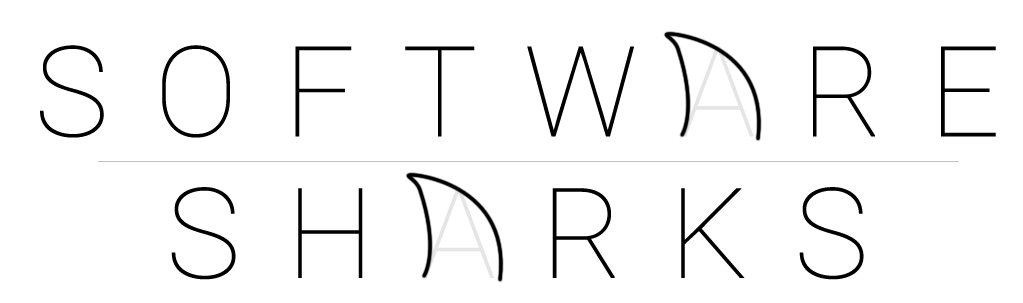
\includegraphics[width=0.5\linewidth]{images/sslogo.png}
	\centering
	
    \scshape
    \sffamily
	
	\vspace*{\baselineskip}
	
	\rule{\textwidth}{3pt}
	
	\vspace{0.75\baselineskip}
	
	\textrm{\LARGE \textbf{Coding Standards} \\ for\\ \systemTitle{}\\ \small Version 1.0.0 - Demo \#5 Final\\}
	
	\vspace{0.75\baselineskip}
	
	\rule{\textwidth}{3pt} 
	
	\vspace{2\baselineskip}
	
	A detailed set of guidelines dictating the best practices, programming styles and conventions that all developers of this project will adhere to. \\ 
    \footnotesize Please note that these guidelines were heavily influenced by the style guides released by Google\footnote{http://google.github.io/styleguide/} under the Creative Commons Licence\footnote{https://creativecommons.org/licenses/by/3.0/}.
	
	\vspace*{3\baselineskip}
	
	Compiled By
	
	\vspace{0.5\baselineskip}
	
    \textsf{\large
    \textrm{\textbf{The Software Sharks Team}} \\
    \small 
    Coetzer MJ \\
    Bester TJ \\
    Orrie O \\
    Lew J \\
    Matodzi MC \\
    } 
	
	\vspace{0.5\baselineskip}
	
	\textit{ Department of Computer Science \\ The University of Pretoria}
	
    \vfill
    \includegraphics[width=0.5\linewidth]{images/uplogo.png}
    \vfill
    For
	
	\vspace{0.5\baselineskip}
	
    \textsf{\large
    \textrm{\textbf{Bramhope International School of Innovation}} \\
    } 

\end{titlepage}

\pagebreak

%----------------------------------------------------------------------------------------
%	COPYRIGHT PAGE
%----------------------------------------------------------------------------------------

\newpage
~\vfill
\thispagestyle{empty}

\noindent COS 301 Team: Software Sharks\\ 

\noindent \textsc{Department of Computer Science, University of Pretoria}\\

\noindent \textsc{https://github.com/OrishaOrrie/SoftwareSharks}\\ % URL

\noindent This coding standards document was drafted under the supervision of involved lecturers according to the assessment guidelines of the final year Computer Science module: COS 301 - Software Engineering, presented by the Department of Computer Science in the faculty of Engineering, Built Environment and Information Technology at the University of Pretoria during the first semester of the year 2018. \\ \\
\textbf{Disclaimer: }This document is a modification of the Google Style Guides licensed under the Creative Commons 3.0 Attribution - Allowing total reuse and modification and as such the Software Sharks, Department of Computer Science nor the University of Pretoria claim this entire document to be their original work. \\ % License information
\includegraphics{images/cc_by.png} \\

\noindent \textit{First release, September 2018} % Edition date

\pagebreak

%----------------------------------------------------------------------------------------
%	Table of Contents
%----------------------------------------------------------------------------------------
\tableofcontents

\pagebreak


%----------------------------------------------------------------------------------------
%	Introduction
%----------------------------------------------------------------------------------------
\section{Introduction}
This is a document defining the coding standards for the Ninshiki system, it defines the rules which govern how the development team members are to code. This includes comments structure, method structure and class structure as well as the various naming conventions. This also contains the GitHub structure used by the team as well as the file headers that are used in each of the software files.

\section{Detailed System design}
\begin{sidewaysfigure}
    \includegraphics[width=\textwidth]{images/ClassDiagram.png}
\end{sidewaysfigure}
The following class diagram, which can be found on the next page, shows all the classes, attributes, operations and relationships between all the objects in the system.
It includes all the components of the App subsystems as well as the Dashboard subsystem.

The diagram can also be found on the following link: \linebreak
\linebreak
\url{https://drive.google.com/open?id=1ds-pWCZJv6vkCVnpeTRlIQAlpgVUn8eO}

\pagebreak

%----------------------------------------------------------------------------------------
%	Code Review Process
%----------------------------------------------------------------------------------------
\section{Code Review Processes}
% Describe how and how often you apply code reviews to confirm adherence to your coding standards. Mention the editors and tools you use and how they should be configured.

\subsection{Github}
All major releases are subjected to peer review before being merged into the master branch as described in the process below:
\begin{enumerate}
    \item Major feature or fix is implemented in it's respective branch
    \item A pull-request is requested to compare the potential changes
    \item The developer then assigns two separate members of the team to the request
    \item These members then review and either approve/decline the request by evaluating the code and functionality and ultimately providing the appropriate reasoning
    \item Depending on the above result the request is either merged into master or declined until the appropriate fixes have been made
\end{enumerate}

\subsection{Informal Reviews}
All interrelated modules and subsystems should be periodically and actively checked to ensure the satisfaction of these coding standards through out the development process.
\begin{enumerate}
    \item Developers are required to review their own code \& functionality
    \item Developers are required to inform respective authors of violations or errors present in their code-base
    \item All potential violations or errors should be stipulated in a Github issue detailing the exact violations or errors to allow for optimal evaluation and potential fixes
\end{enumerate}

\pagebreak
\section{Github Repository Structure}
The Software Sharks GitHub repository can be found at the following location:
\url{https://github.com/OrishaOrrie/SoftwareSharks}

This section describes the structure of this repository, specifically the current master branch.

\begin{tabbing}
	
|-App\=lic\=ati\=on\=Sou\=rce\= \\
\>| -  Backend\\
\>\>|- Node Server\\
\> \> \> |--functions\\
\>\>|- Image Scraper\\
\>\>|- Keras Training Model\\
\> \> \> |-- tests\\
\> \>|-- Firebase Admin \\

\>| - Mobile/ \\
\>\>|--latest APK\\
\>\>|--myApp\\
\>\>\>|--.sourcemaps\\
\>\>\>|--resources\\
\>\>\>\>\>|--Android\\
\>\>\>|--src\\
\>\>\>\>\>|--app\\
\>\>\>\>\>|--assets/imgs\\
\>\>\>\>\>|--pages\\
\>\>\>\>\>\>|--about\\
\>\>\>\>\>\>|--contact\\
\>\>\>\>\>\>|--home\\
\>\>\>\>\>\>|--imagerec\\
\>\>\>\>\>\>|--results\\
\>\>\>\>\>\>|--tabs\\
\>\>\>\>\>\>|--utilities\\
\>\>\>\>\>|--provider/model-loader\\
\>| - ss-imagerecc-webapp\\
\>\>|-- dist/ \\
\>\>|-- documentation/ \\
\>\>|-- e2e/ \\
\>\>|-- functions/ \\
\>\>|-- node\_modules/ \\
\>\>|-- src/ (O)\\
\>\>\>|-- app\\
\>\>\>\>\>|-- contact-us\\
\>\>\>\>\>\>|-- contact-us.component.css\\
\>\>\>\>\>\>|-- contact-us.component.html\\
\>\>\>\>\>\>				|-- contact-us.component.spec.ts\\
\>\>\>\>\>\>				|-- contact-us.component.ts\\
\>\>\>\>\>			|-- home/\\
\>\>\>\>\>				|-- imageupload/\\
\>\>\>\>\>			|-- utilities/\\
\>\>\>\>\>				|-- app.component.css (P)\\
\>\>\>\>\>				|-- app.component.html\\
\>\>\>\>\>				|-- app.component.spec.ts\\
\>\>\>\>\>			|-- app.component.ts\\
\>\>\>		|-- assets/ \\
\>\>\>		|-- environments/ \\
\>\>\>		|-- index.html \\
\>\>\>		|-- styles.css \\
\>\>\>		|-- test.ts \\
\>\>	|-- package.json \\
\>\>	|-- package-lock.json\\
\>\>	|-- firebase.json \\
\>\>	|-- protractor.conf.js \\
\>\>	|-- angular.json \\
\>|-- .gitignore \\
| - Documentation/ \\
| - docs/ \\
     \>| -  css\\
     \>| -  img\\
     \>| -  js\\
     \>| -  mail\\
     \>| -  vendor\\
\end{tabbing}


The root folder contains two folders, Documentation and Application Source, and a Readme file.

The Documentation folder contains references for the project, from the User Manual to the Requirements Specification.
The Readme file provides a concise description of the project, the project management structure, and the Software Sharks team.

The Application Source folder contains the entirety of the software source code, including unit tests and installation scripts.

Each subsystem has its own folder in the Application Source folder, which also includes the dependency and installation batch files.

\pagebreak
%----------------------------------------------------------------------------------------
%	General Coding Conventions
%----------------------------------------------------------------------------------------
\section{Software Sharks General Coding Conventions}
%----------------------------------------------------------------------------------------
%	HTML / CSS
%----------------------------------------------------------------------------------------
\subsection{File Headers}
This section describes the Ninshiki program header template. This header is used as a standardized approach to describing the metadata/functional details of a class.

This header can be found in each of the main classes for each subsystem’s application source.
The following template is used for the header:
\begin{itemize}
\item File Name - Name of class/file.
\item Version Number
\item Author Name
\item Project Name - Ninshiki
\item Organization - Software Sharks
\item Update History - A table containing the version number, date, author, and update description.
\item Functional Description - A brief description of the use cases that the class completes.
\item Related Classes - Classes that assist this class in completing its use cases.
\end{itemize}
\pagebreak


\subsection{HTML/CSS}
\subsubsection{General Style Rules}
\paragraph{Protocol}
\begin{itemize}
\item Never omit the protocol when embedding a resource, image or script.
\item Always make use of the HTTPS protocol for embedding resources, images or scripts when available. 
\end{itemize}

\begin{minted}{html}
<!-- Recommended -->
<script src="https://example.com/example/someJava.min.js"></script>
\end{minted}

\subsubsection{General Formatting Rules}

\paragraph{Indentation}
\begin{itemize}
\item Indent with two spaces.
\item Do not make use of tabs or various spacing other than the above for indentation.
\end{itemize}
\begin{minted}{html}
<!-- Recommended -->
<ul>
␣␣<li>Item 1
␣␣<li>Random Item 2
</ul>
\end{minted}

\paragraph{Capitalisation}
\begin{itemize}
\item All code has to be in lower-case with the exception of strings.
\end{itemize}
\begin{minted}{html}
<!-- Recommended -->
<img src="google.png" alt="Google">
\end{minted}

\paragraph{Trailing White Space}
\begin{itemize}
\item Ensure that there are no trailing white spaces in any line.
\end{itemize}

\pagebreak

\subsubsection{General Meta Rules}

\paragraph{Encoding}
\begin{itemize}
\item Make use of UTF-8 encoding that does not include a byte order mark.
\item Specify the encoding in HTML templates and documents via \mint{html}|<meta charset="utf-8">|
\item Do not specify the encoding of style sheets as these assume UTF-8.
\end{itemize}

\paragraph{Comments}
\begin{itemize}
\item Where ever possible explain code as needed.
\item Use comments to explain code: What does it cover, what purpose does it serve, why is respective solution used or preferred?
\end{itemize}

\paragraph{Action Items}
\begin{itemize}
\item Mark todos and action items with \mintinline{fancy}{TODO}.
\item Highlight todos by using the keyword \mintinline{fancy}{TODO} only, not other common formats like \mintinline{fancy}{@@}.
\item Append a contact (username or mailing list) in parentheses as with the format \mintinline{fancy}{TODO(contact)}.
\item Append action items after a colon as in \mintinline{fancy}{TODO: action item}.
\end{itemize}
\begin{minted}{html}
<!-- TODO: remove optional tags -->
<ul>
  <li>Tag 1</li>
  <li>Tag 2 (Optional)</li>
</ul>
\end{minted}

\pagebreak

\subsection{HTML}

\subsubsection{HTML Style Rules}

\paragraph{Document Type}
\begin{itemize}
\item Use HTML5.
\item HTML5 (HTML syntax) is preferred for all HTML documents: \mintinline{html}{<!DOCTYPE html>}.
\item Do not close void elements, i.e. write \mintinline{html}{<br>}, not \mintinline{html}{<br />}.
\end{itemize}

\paragraph{HTML Validity}
\begin{itemize}
\item Use valid HTML where possible according to the W3C\footnote{https://validator.w3.org/nu/}.
\item Use valid HTML code unless that is not possible due to otherwise unattainable performance goals regarding file size.
\end{itemize}

\paragraph{Semantics}
\begin{itemize}
\item Use elements (sometimes incorrectly called “tags”) for what they have been created for. For example, use heading elements for headings, \mintinline{html}{<p>} elements for paragraphs, \mintinline{html}{<a>} elements for anchors, etc.
\end{itemize}

\paragraph{Multimedia Fall-back}
\begin{itemize}
\item For multimedia (such as images, videos and animated objects via \mintinline{html}{<canvas>}) make sure to provide meaningful alternative text via \mintinline{html}{alt="Descriptive alt text"} to enable global accessibility.
\end{itemize}
\begin{minted}{html}
<!-- Recommended -->
<img src="spreadsheet.png" alt="Spreadsheet screenshot.">
\end{minted}

\paragraph{Separation of Concerns}
\begin{itemize}
\item Separate structure (HTML), presentation (CSS) and behaviour (Scripts) into their respective files and file-types.
\end{itemize}

\paragraph{Entity References}
\begin{itemize}
\item Do not make use of entity references except for special HTML characters (< and \&).
\end{itemize}

\paragraph{\mintinline{html}{type} Attributes}
\begin{itemize}
\item Do not use \mintinline{html}{type} attributes for style sheets (unless not using CSS) and scripts (unless not using JavaScript).
\end{itemize}
\begin{minted}{html}
<!-- Recommended -->
<link rel="stylesheet" href="https://www.google.com/css/maia.css">
<script src="https://www.google.com/js/gweb/analytics/autotrack.js"></script>
\end{minted}

\subsubsection{HTML Formatting Rules}

\paragraph{General Formatting}
\begin{itemize}
\item Use a new line for every block, list or table element.
\item Indent every such child element.
\end{itemize}

\paragraph{HTML Line-Wrapping}
\begin{itemize}
\item It is optional to break long lines in order to improve readability.
\item If lines are broken then the continuation line should be indented at least 4 additional spaces from the original line.
\end{itemize}

\paragraph{HTML Quotation Marks}
\begin{itemize}
\item When quoting attribute values, make use of double quotation marks instead of single quotation marks.
\end{itemize}
\begin{minted}{html}
<!-- Recommended -->
<a class="maia button-secondary">Sign in</a>
\end{minted}

\pagebreak

\subsection{CSS}

\subsubsection{CSS Style Rules}

\paragraph{CSS Validity}
\begin{itemize}
\item Use valid CSS where possible according to the W3C\footnote{https://jigsaw.w3.org/css-validator/}.
\end{itemize}

\paragraph{ID and Class Naming}
\begin{itemize}
\item Use meaningful or generic ID and class names that clearly reflect the purpose of the element instead of presentational or cryptic names.
\end{itemize}
\begin{minted}{css}
/* Recommended: specific */
#gallery {}
#login {}
.video {}

/* Recommended: generic */
.aux {}
.alt {}
\end{minted}

\paragraph{ID and Class Name Style}
\begin{itemize}
\item Use ID and class names that are as short as possible but as long as necessary.
\end{itemize}

\paragraph{Type Selectors}
\begin{itemize}
\item Avoid qualifying ID and class names with type selectors.
\end{itemize}

\paragraph{Shorthand Properties}
\begin{itemize}
\item Use shorthand properties where possible for code efficiency and understandability.
\end{itemize}

\paragraph{Leading 0s}
\begin{itemize}
\item Omit leading “0”s in values or lengths between -1 and 1.
\end{itemize}
\begin{minted}{css}
/* Recommended */
font-size: .8em;
\end{minted}

\paragraph{Hexadecimal Notation}
\begin{itemize}
\item Use 3 character hexadecimal notation where possible.
\end{itemize}
\begin{minted}{css}
/* Recommended */
color: #ebc; /* Instead of #eebbcc */
\end{minted}

\paragraph{ID and Class Name Delimiters}
\begin{itemize}
\item Separate words in ID and class names by a hyphen only.
\end{itemize}
\begin{minted}{css}
/* Recommended */
#video-id {}
.ads-sample {}
\end{minted}

\subsubsection{CSS Formatting Rules}

\paragraph{Declaration Order}
\begin{itemize}
\item Alphabetize declarations in order to achieve consistent code in a way that is easy to remember and maintain.
\item Ignore vendor-specific prefixes.
\end{itemize}

\paragraph{Block Content Indentation}
\begin{itemize}
\item Indent all block content so to reflect hierarchy and improve understanding.
\end{itemize}

\paragraph{Declaration Stops}
\begin{itemize}
\item End every declaration with a semicolon for consistency and extensibility reasons.
\end{itemize}

\paragraph{Property Name Stops}
\begin{itemize}
\item Use a space after a property name’s colon but not before.
\end{itemize}

\paragraph{Declaration Block Separation}
\begin{itemize}
\item Always use a single space between the last selector and the opening brace that begins the declaration block.
\end{itemize}
\begin{minted}{css}
/* Recommended */
#video {
  margin-top: 1em;
}
\end{minted}

\paragraph{Selector and Declaration Separation}
\begin{itemize}
\item Separate selectors and declarations by new lines.
\end{itemize}
\begin{minted}{css}
/* Recommended */
h1,
h2,
h3 {
  font-weight: normal;
  line-height: 1.2;
}
\end{minted}

\paragraph{Rule Separation}
\begin{itemize}
\item Separate rules by a blank line.
\end{itemize}

\paragraph{CSS Quotation Marks}
\begin{itemize}
\item Use single ( \mintinline{css}{''} ) rather than double ( \mintinline{css}{""} ) quotation marks for attribute selectors and property values.
\item Do not use quotation marks in URI values (\mintinline{css}{url()}).
\end{itemize}
\begin{minted}{css}
/* Recommended */
@import url(https://www.google.com/css/maia.css);

html {
  font-family: 'open sans', arial, sans-serif;
}
\end{minted}

\subsubsection{CSS Meta Rules}

\paragraph{Section Comments}
\begin{itemize}
\item If possible, group style sheet sections together by using comments. Separate sections with new lines.
\end{itemize}
\begin{minted}{css}
/* Recommended */
/* Header */

#adw-header {}

/* Footer */

#adw-footer {}
\end{minted}

\pagebreak

%----------------------------------------------------------------------------------------
%	JavaScript
%----------------------------------------------------------------------------------------
\subsection{JavaScript}
\subsubsection{File Name}
\begin{itemize}
\item File names must be all lower-case and may include underscores (\_) or dashes (-), but no additional punctuation.
\item Follow the convention that your project uses. 
\item File name extensions must be '\mintinline{fancy}{.js}'.
\end{itemize}

\subsubsection{File Encoding}
\begin{itemize}
\item All source files must be encoded in UTF-8.
\end{itemize}

\subsubsection{Special Characters}

\paragraph{Whitespace Characters}
\begin{itemize}
\item Aside from the line terminator sequence, the ASCII horizontal space character (0x20) is the only whitespace character that appears anywhere in a source file.
\item All other whitespace characters in string literals are escaped.
\item Tab characters are not used for indentation.
\end{itemize}

\paragraph{Special escape sequences}
\begin{itemize}
\item Use special escape sequences: \mintinline{JavaScript}{" \', \", \\, \b, \f, \n, \r, \t, \v "}.
\item Do not use numeric or octal escapes.
\end{itemize}

\subsubsection{Source File Structure}
A source file consists of, in order:
\begin{enumerate}
\item Licence or copyright information if available.
\item \mintinline{JavaScript}{// @fileoverview} JSDoc.
\item File implementation.
\end{enumerate}
Exactly one blank line separates each section that is present.

\subsubsection{Formatting}

\paragraph{Braces}

\paragraph{Braces are Used for all Control Structures}
\begin{itemize}
\item Braces are required for all control structures.
\item The first statement of a non-empty block must begin on its own line.
\end{itemize}

\paragraph{Non-empty blocks: K\&R style\\}
Braces follow the Kernighan and Ritchie style ("Egyptian brackets") for non-empty blocks and block-like constructs:
\begin{itemize}
\item No line break before the opening brace.
\item Line break after the opening brace.
\item Line break before the closing brace.
\item Line break after the closing brace if that brace terminates a statement or the body of a function or class statement, or a class method. 
\end{itemize}
\begin{minted}{JavaScript}
class InnerClass {
  constructor() {}

  /** @param {number} foo */
  method(foo) {
    if (condition(foo)) {
      try {
        // Note: this might fail.
        something();
      } catch (err) {
        recover();
      }
    }
  }
}
\end{minted}

\paragraph{Empty blocks: may be concise}
\begin{itemize}
\item An empty block or block-like construct may be closed immediately after it is opened, with no characters, space, or line break in between.
\end{itemize}

\paragraph{Block indentation: +2 spaces}

\paragraph{Array literals: optionally "block-like"}

%----------------------------------------------------------------------------------------
%	Python
%----------------------------------------------------------------------------------------
\newpage
\subsection{Python}
\subsubsection{Python Style Rules}
\paragraph{Semi-colons}
\begin{itemize}
\item  Do not terminate your lines with semi-colons and do not use semi-colons to put two commands on the same line.
\end{itemize}
\paragraph{Line length}
\begin{itemize}
\item  Maximum line length is 80 characters.
\item Exceptions: 
\begin{itemize}
\item Long import statements.
\item URLs in comments.
\end{itemize}
\item Do not use backslash line continuation.
\item Make use of Python's implicit line joining inside parentheses, brackets and braces. If necessary, you can add an extra pair of parentheses around an expression.
\item When a literal string won't fit on a single line, use parentheses for implicit line joining.
\item Within comments, put long URLs on their own line if necessary.
\begin{minted} {python}
Yes:  # See details at
      # https://www.example.com/us/developer/documentation/api/content/v2.0/csv_file_name_extension_full_specification.html
\end{minted}
\end{itemize}

\paragraph{Parenthesis}
\begin{itemize}
\item Use parentheses sparingly.
Do not use them in return statements or conditional statements unless using parentheses for implied line continuation. It is however fine to use parentheses around tuples.
\begin{minted} {python} 
Yes: if foo:
         bar()
     while x:
         x = bar()
     if x and y:
         bar()
     if not x:
         bar()
     return foo
     for (x, y) in dict.items(): ...
\end{minted}
\begin{minted} {python}
No:  if (x):
         bar()
     if not(x):
         bar()
     return (foo)
\end{minted}

\end{itemize}


\paragraph{Indentation}
\begin{itemize}
\item Indent your code blocks with 4 spaces.
\item Never use tabs or mix tabs and spaces. In cases of implied line continuation, you should align wrapped elements either vertically, as per the examples in the line length section; or using a hanging indent of 4 spaces, in which case there should be no argument on the first line.
\begin{minted} {python}
Yes:   # Aligned with opening delimiter
       foo = long_function_name(var_one, var_two,
                                var_three, var_four)

       # Aligned with opening delimiter in a dictionary
       foo = {
           long_dictionary_key: value1 +
                                value2,
           ...
       }

       # 4-space hanging indent; nothing on first line
       foo = long_function_name(
           var_one, var_two, var_three,
           var_four)

       # 4-space hanging indent in a dictionary
       foo = {
           long_dictionary_key:
               long_dictionary_value,
           ...
       }

\end{minted}
\end{itemize}


\paragraph{Blank Lines}
\begin{itemize}
\item Two blank lines between top-level definitions, one blank line between method definitions.
\item Two blank lines between top-level definitions, be they function or class definitions. 
\item One blank line between method definitions and between the class line and the first method. Use single blank lines as you judge appropriate within functions or methods.
\end{itemize}

\paragraph{Whitespace}
\begin{itemize}
\item Follow standard typographic rules for the use of spaces around punctuation.
\item No whitespace inside parentheses, brackets or braces.

\item No whitespace before a comma, semicolon, or colon. Do use whitespace after a comma, semicolon, or colon except at the end of the line.
\begin{minted} {python}
Yes: if x == 4:
         print x, y
     x, y = y, x
\end{minted}

\item No whitespace before the open paren/bracket that starts an argument list, indexing or slicing.

\item Surround binary operators with a single space on either side for assignment (=), comparisons (==, <, >, !=, <>, <=, >=, in, not in, is, is not), and Boolean (and, or, not). Use your better judgement for the insertion of spaces around arithmetic operators but always be consistent about white-space on either side of a binary operator.

\item Don't use spaces around the '=' sign when used to indicate a keyword argument or a default parameter value.
\begin{minted} {python}
Yes: def complex(real, image =0.0): return magic(r=real, i=image)
\end{minted}

\item Don't use spaces to vertically align tokens on consecutive lines, since it becomes a maintenance burden (applies to :, =, etc.):
\begin{minted} {python}
Yes:
  foo = 1000  # comment
  long_name = 2  # comment that should not be aligned

  dictionary = {
      'foo': 1,
      'long_name': 2,
  }
\end{minted}
\end{itemize} 
\section{Global Style Rules}
The following list contains links to Google Style rules for each language used which the code will also loosely adhere to:
\begin{itemize}
\item HTML and CSS: \url{https://google.github.io/styleguide/htmlcssguide.html}
\item JavaScript: \url{https://google.github.io/styleguide/javascriptguide.xml}
\item Python: \url{https://github.com/google/styleguide/blob/gh-pages/pyguide.md}

\end{itemize}
\end{document}
